% !TeX spellcheck = en_GB

\documentclass[a4paper,12pt]{article}


\usepackage{alltt, fancyvrb, url}
\usepackage{graphicx}
\usepackage{subfigure}
\usepackage{wrapfig}
\usepackage{algorithmic}
\usepackage[utf8]{inputenc}
\usepackage{fontenc}
\usepackage{amsmath,stmaryrd,mathtools,algorithm}
\usepackage{amssymb}
\usepackage{longtable}
\usepackage{multirow}
\usepackage{setspace}
\usepackage{todonotes}
\usepackage{csquotes}
\usepackage[margin=1.05in]{geometry}
\usepackage{todonotes}

% Remove option to use English naming
\usepackage[colorlinks,
	linkcolor={red!70!black},
	citecolor={blue!80!black},
	urlcolor={blue!50!black}]{hyperref}
\usepackage[nameinlink]{cleveref}

\usepackage{xcolor}
\usepackage{textcomp}
\usepackage{listings}


\definecolor{myPink}  {rgb}{0.67, 0.05, 0.57} % keywords
\definecolor{myRed}   {rgb}{0.87, 0.20, 0.00} % strings
\definecolor{myGreen} {rgb}{0.00, 0.47, 0.00} % comments
\definecolor{myBrown} {rgb}{0.39, 0.22, 0.13} % brown

\lstdefinestyle{Xcode} {
	language        = C,
	basicstyle      = \footnotesize\ttfamily,
	identifierstyle = \color{black},
	commentstyle    = \color{myGreen},
	keywordstyle    = \color{myPink},
	stringstyle     = \color{myRed},
	directivestyle  = \color{myBrown},
	extendedchars   = true,
	tabsize         = 4,
	showspaces      = false,
	showstringspaces = false,
	breakautoindent = true,
	flexiblecolumns = true,
	keepspaces      = true,
	stepnumber      = 1,
	xleftmargin     = 0pt,
	numbers=left
}

\lstset{
	style=Xcode,
	%caption=lstname,
	breaklines=false,
	frame=single
}

\title{Data visualization -- Process Book\\\textbf{Work in progress}}
\setcounter{tocdepth}{3}
\setcounter{secnumdepth}{3}
 
\author{Dario Pavllo \and Niccolò Sacchi \and Mattia Martinelli}
\date{} %\today

\begin{document}
\pagenumbering{arabic}
\maketitle
\section{Introduction}
Buying from huge e-commerce websites such as \emph{Amazon} has many advantages, but paradoxically, users are often confused by the vast variety of products that are offered. Users may have a rough idea about the characteristics of the product they want to buy, but they often undergo the same process of comparing similar products. We aim to remove this redundancy and aid them in their purchases, suggesting the best or most popular products that correspond to their search. For instance, comparing smartphones or laptops may be difficult due to the wide price range and the required technical knowledge. With our platform, customers can easily visualise in a graphical way what products match their needs, and among them, the most popular and favourite ones.

\subsection{Idea and related work}
Amazon's website already offers a sophisticated search system, which allows users to select category, price range and some technical characteristics of the product they want to buy. But would it not be nice to query among similar articles without explicitly providing to the website such features? For instance, product description  \href{https://www.amazon.com/Acer-E5-575-33BM-15-6-Inch-Notebook-Generation/dp/B01K1IO3QW/ref=sr_1_3?s=pc&ie=UTF8&qid=1512207600&sr=1-3&keywords=laptop}{pages} already contain relevant information about related articles, such as \textit{similar items}, \textit{items bought together} and \textit{items that customers buy after viewing this item}. These links suggest alternatives to the customer; however, they only show \textit{neighbouring} offers and not the whole overview of offers. To overcome this limitation, we have decided to develop a graphical and interactive visualization that shows such relations among multiple articles. If products are showed as a network, as pictured in \Cref{fig:graphNav}, it is clear to see which ones users usually end up buying. Imagine a user who wishes to buy some professional studio headphones and has a rough idea of their characteristics. By querying the graph, he/she can highlight relevant products and follow the highlighted path towards an optimal product. Of course, defining what articles may be \emph{optimal} is not a trivial task; however, if many clients buy the same product after reviewing a set of other products, then it is very likely that the former is more appealing. In addition, there are groups of products in which there is no preferred product, i.e. users do not show great propensity in buying one of them. Each one of these groups represent a cluster of competing products and the choice of the best one depends on the metric chosen by the user. \todo{the role of cliques must be better defined}
\begin{figure}[H]
	\centering{}
	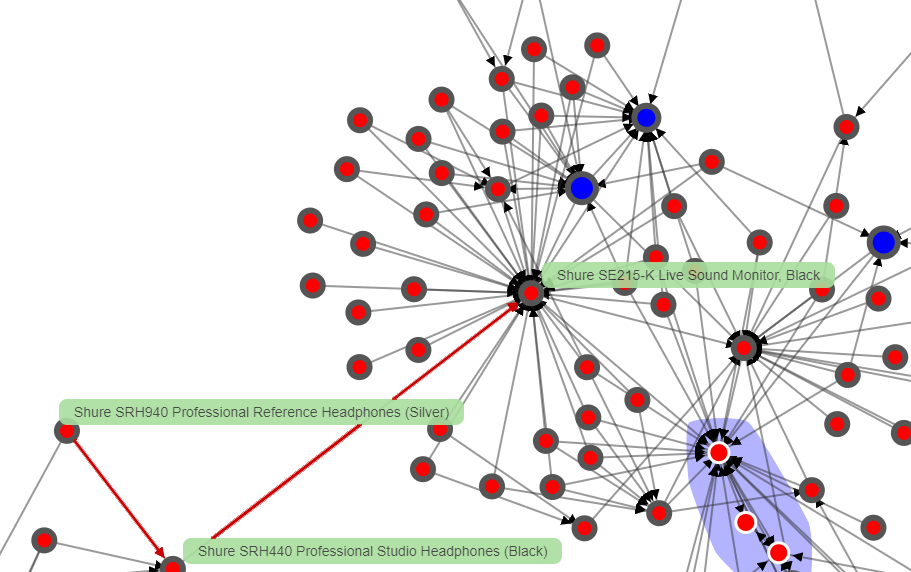
\includegraphics[width=\textwidth]{img/graph_nav.png}
	\caption{Subgraph of the \emph{Headphones} category. As can be seen, some nodes (products) are \emph{attractors}, in the sense that users end up buying those after reviewing a large number of other products.}
	\label{fig:graphNav}
\end{figure}

\section{Dataset}
We have been provided with a dataset of \href{http://jmcauley.ucsd.edu/data/amazon/}{Amazon products} that contains relations among the articles, such as ``bought together'', ``also viewed'', and/or ``buy after viewing''. These links reflect the behaviour of users that buy on the website, therefore, they are used to create our graph.
% What about this part?
%These relations will be used for creating a graph that represents competing products with similar characteristics, i.e. products that are viewed together but not bought together. Our assumption is that people interested in a certain product would have visualized and compared similar products prior to buying whichever they consider the best.

\section{The graph}
The graph is built by adding an edge between product A and product B if B is bought after viewing A. Conversely, if two products are frequently bought together, we remove the edge between them since they can not be considered as competing with eachother (e.g. a cover and a smartphone). In our context, a directed edge from A to B means ``B is preferred over A``, whereas an undirected edge (or, equivalently, two opposite directed edges) means ``A is competing with B''.

It is easy to extend this definition to groups of competing products, that is, max-cliques. If some groups are totally interconnected, we can assume that they are in direct competition and that one is not necessarily better than the other. \todo{Review connected components and how they are made}

\section{Visualization}

\begin{figure}[H]
	\centering{}
	
\includegraphics[width=\textwidth]{img/amazon.png}
	\caption{Introductory screen of the webpage.}
	\label{fig:amazon}
\end{figure}
In summary, the visualization guides the user from their idea of product to the final result. In particular, the process should be as follows:

\begin{enumerate}
	\item The user is presented with a selector that navigates through the Amazon category tree (\Cref{fig:category}), and allows him/her to select a category (e.g. headphones, mobile phones, laptops, etc.). Of course, it will also be possible to search for a category according to some keywords.
	\begin{figure}[H]
		\centering{}
		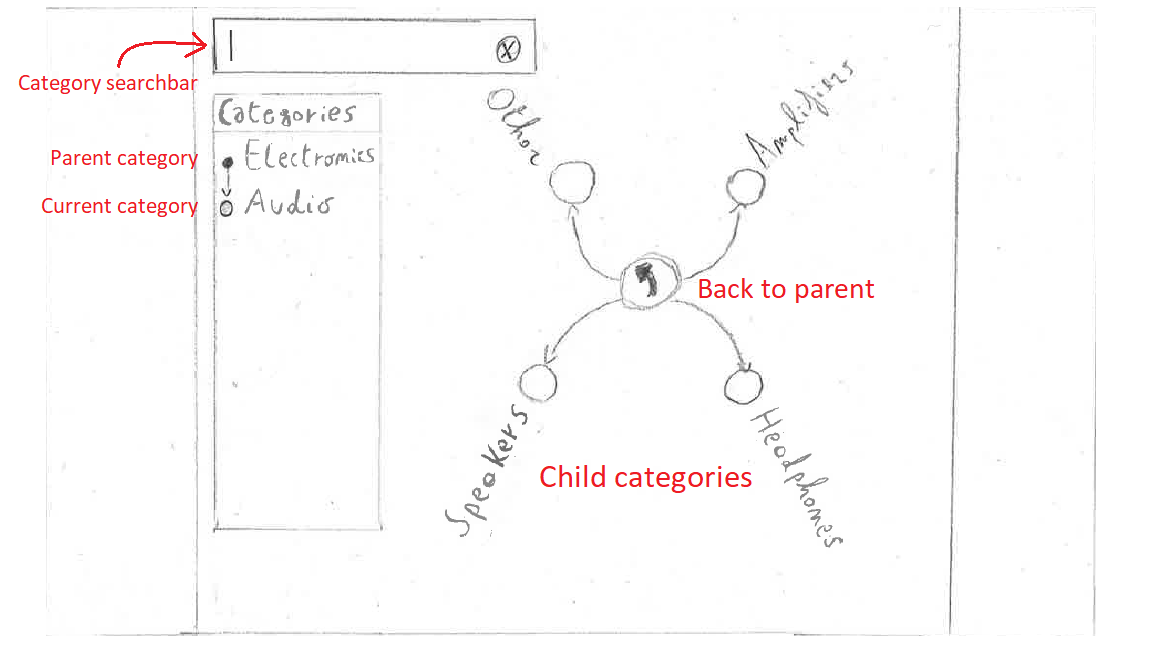
\includegraphics[width=\textwidth]{img/categories.png}
		\caption{Category navigation.}
		\label{fig:category}
	\end{figure}
	\item Once a category is selected, the graph view appears (\Cref{fig:graph}). Initially, the full graph is shown, so that the user can get a sense of its topology (sparseness, attractors, cliques, etc.).
		\begin{figure}[H]
		\centering{}
		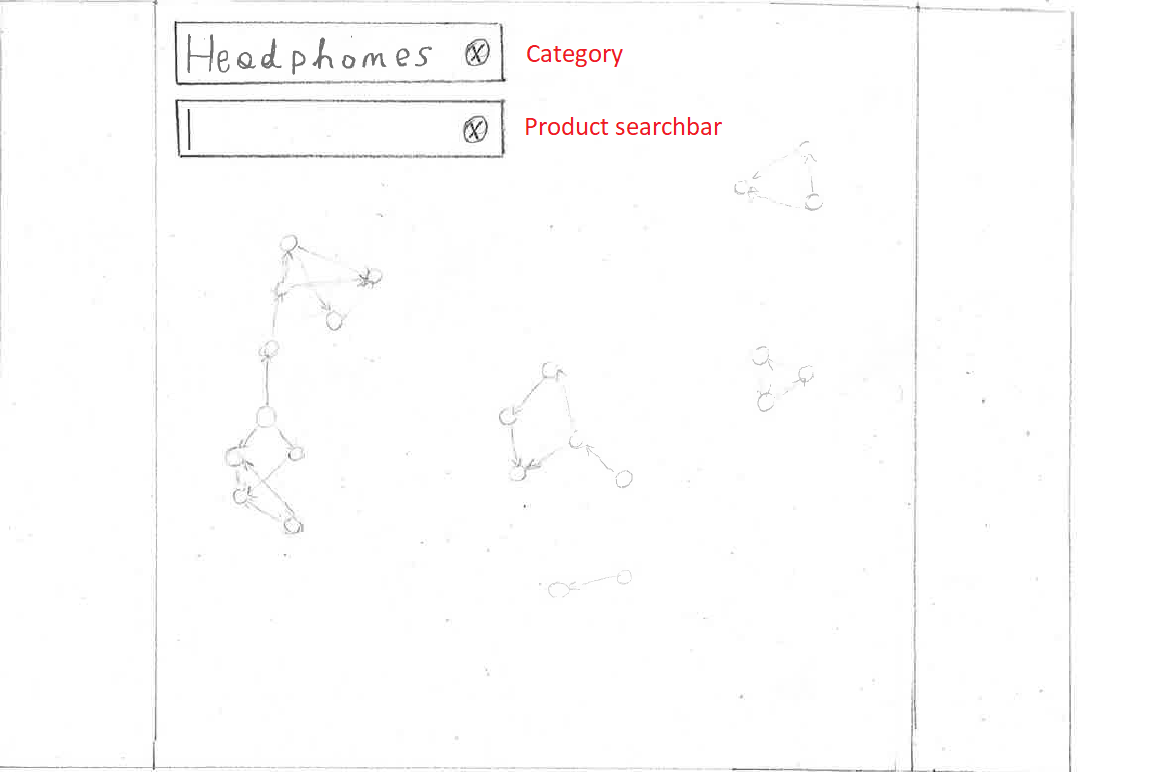
\includegraphics[width=\textwidth]{img/graph.png}
		\caption{The whole graph is shown when a category is selected.}
		\label{fig:graph}
	\end{figure}
	\item The user can query a few keywords and set a price range, which will cause the graph to highlight only relevant parts and collapse the rest. At this point, the user can inspect the paths between products, as well as the \emph{attractors}. The visualization will also provide some recommendations (automatic paths) and display the characteristics of the products, along with their differences.
		\begin{figure}[H]
		\centering{}
		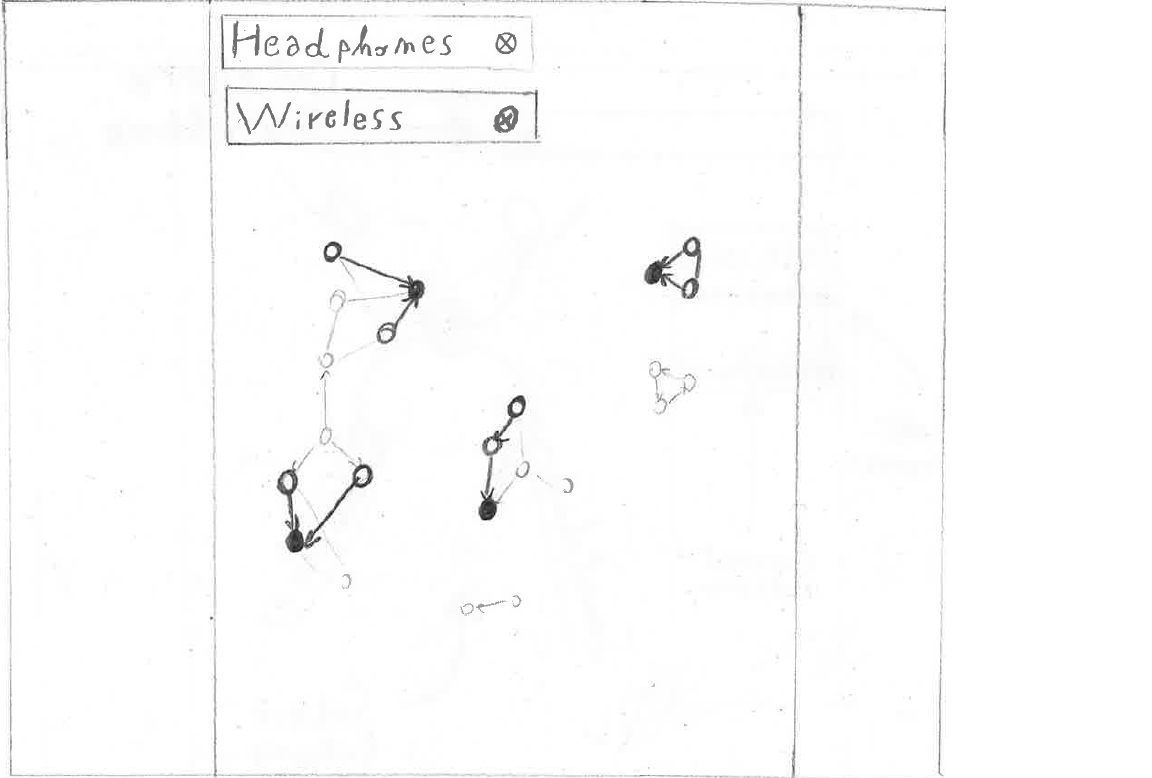
\includegraphics[width=\textwidth]{img/wireless.png}
		\caption{Example of products filtered according to keyword.}
		\label{fig:wireless}
	\end{figure}
	\item The user can query a few keywords and set a price range, which will cause the graph to highlight only relevant parts and collapse the rest. At this point, the user can inspect the paths between products, as well as the \emph{attractors}. 
	\begin{figure}[H]
	\centering{}
	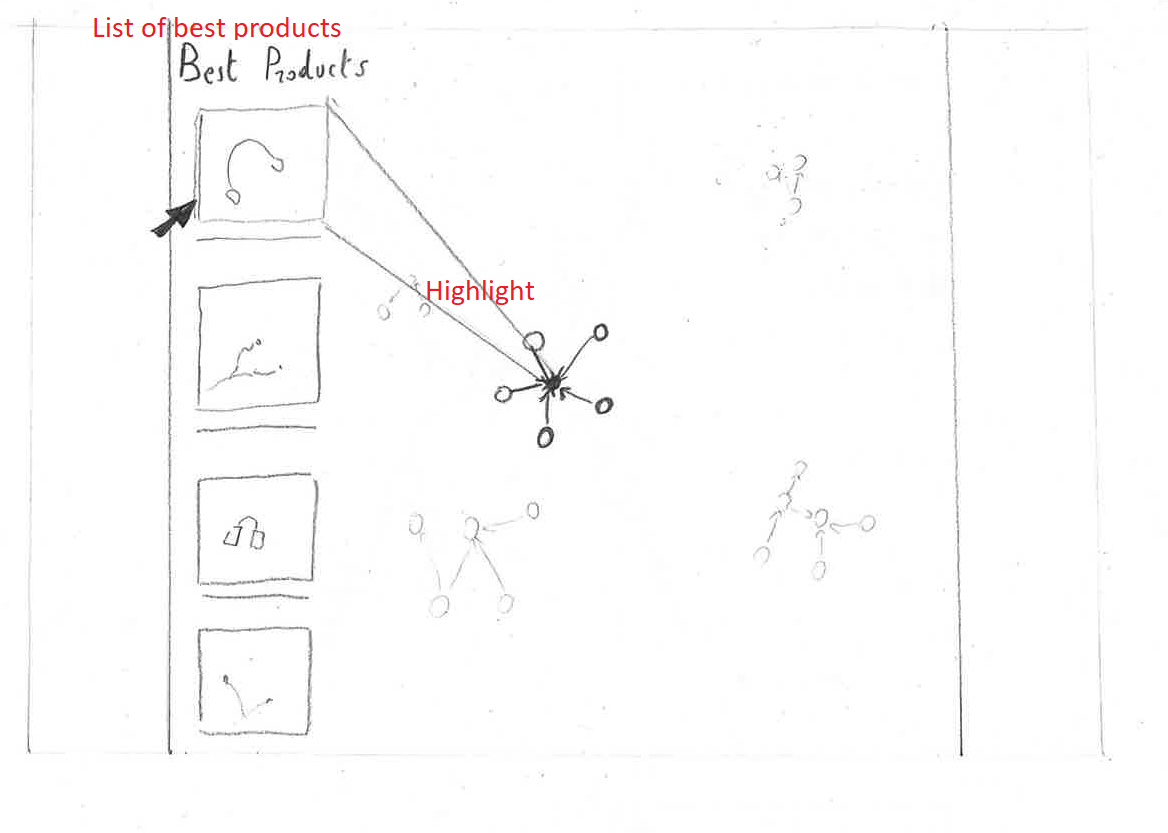
\includegraphics[width=\textwidth]{img/best.png}
	\caption{Best products are directly shown to users, but they are also highlighted on the graph.}
	\label{fig:best}
	\end{figure}
	The visualization provides some recommendations, showing their title, picture and a brief summary of their characteristics. Such recommendations are \textit{attractors}, that is, nodes with the highest incoming edges. Therefore, they are considered the most popular products in category.
\end{enumerate}
\todo{insert additional view with products on the side}
\section{Process}
The graph must show to users the most relevant products in an intuitive manner. As a crucial requirement, users should find the information of interest "at first glance", without need to interpret the graph.
\begin{enumerate}
	\item We opted for \href{http://bl.ocks.org/GerHobbelt/3071239}{this} collapsible graph which would allow to "hide" all the competing products in one node and expand it only if the user is really interested in analazying them. 
	\item Once we display all the products of a category the next step is to choose an intuitive and easy way to select only the parts of the graph in which the user is interested. A simple search box and more advanced visualization (e.g. highlight the path to the bests products, show a list of computed best products, photos and links to the products) will accomplish the task.
	\todo{this whole part must be reviewed. chronological steps must be added}
\end{enumerate}
 

\end{document}
